% Тут используется класс, установленный на сервере Papeeria. На случай, если
% текст понадобится редактировать где-то в другом месте, рядом лежит файл matmex-diploma-custom.cls
% который в момент своего создания был идентичен классу, установленному на сервере.
% Для того, чтобы им воспользоваться, замените matmex-diploma на matmex-diploma-custom
% Если вы работаете исключительно в Papeeria то мы настоятельно рекомендуем пользоваться
% классом matmex-diploma, поскольку он будет автоматически обновляться по мере внесения корректив
%

% По умолчанию используется шрифт 14 размера. Если нужен 12-й шрифт, уберите опцию [14pt]
\documentclass[14pt]{matmex-diploma-custom}
%\documentclass[14pt]{matmex-diploma-custom}

\begin{document}
% Год, город, название университета и факультета предопределены,
% но можно и поменять.
% Если англоязычная титульная страница не нужна, то ее можно просто удалить.
\filltitle{ru}{
    chair              = {Направление Математики и механики\\ Программная инженерия},
    title              = {Цифровая обработка изображений в микроскопии},
    % Здесь указывается тип работы. Возможные значения:
    %   coursework - Курсовая работа
    %   diploma - Диплом специалиста
    %   master - Диплом магистра
    %   bachelor - Диплом бакалавра
    type               = {diploma},
    position           = {студента},
    group              = 471,
    author             = {Кутуев Владимир Александрович},
    supervisorPosition = {ст. преп.},
    supervisor         = {Кириленко Я.\,А.},
    reviewerPosition   = {ст. преп.},
    reviewer           = {Привалов А.\,И.},
    % chairHeadPosition  = {д.\,ф.-м.\,н., профессор},
    % chairHead          = {Хунта К.\,Х.},
%   university         = {Санкт-Петербургский Государственный Университет},
%   faculty            = {Математико-механический факультет},
%   city               = {Санкт-Петербург},
%   year               = {2013}
}

\maketitle
\tableofcontents
% У введения нет номера главы
\section*{Введение}
В микроскопии очень важно получать изображения, на которых различимы все мелкие детали. Но достичь этого исключительно средствами оптики микроскопа не всегда возможно: у объёмных препаратов при большом увеличе    нии с помощью микроскопа можно сфокусироваться только на ограниченные области исследуемого объекта, рассеянный свет из областей находящихся вне зоны фокуса влечет появление различных артефактов, влияющих на чё    ткость изображения. Для повышения качества получаемых изображений было решено создать библиотеку алгоритмов обработки изображений, которая позволит исправить недостатки получаемых цифровой камерой с микроскопа изображений.
\par
В совревременном мире большую популярность приобрели мобильные платформы, поэтому важным требованием является поддержка платформ Android и IOS. Также важно, чтобы решение работало достаточно быстро, сохраняя качество, удовлетворяющее человека.

\section{Focus stacking(focal stacking)}
Для получения резкого изображения плоского препарата достаточно подобрать расстояние фокусировки, при котором всё изображение попадает в фокус. Однако сделать также с объёмными объектами нельзя, так как глубина резкости ограничена, и сфокусированными получаются только определённые области препарата. Для решения этой проблемы применяется техника focus stacking: производится захват серии изображений при разных уровнях фокуса, затем для какждого изображения обределяются наиболее сфокусированные участки, из которых формируется изображение, в котором все области попадают в фокус (рис. \ref{focus_stacking1}).

\begin{figure}[h]
\label{focus_stacking1}
\centering
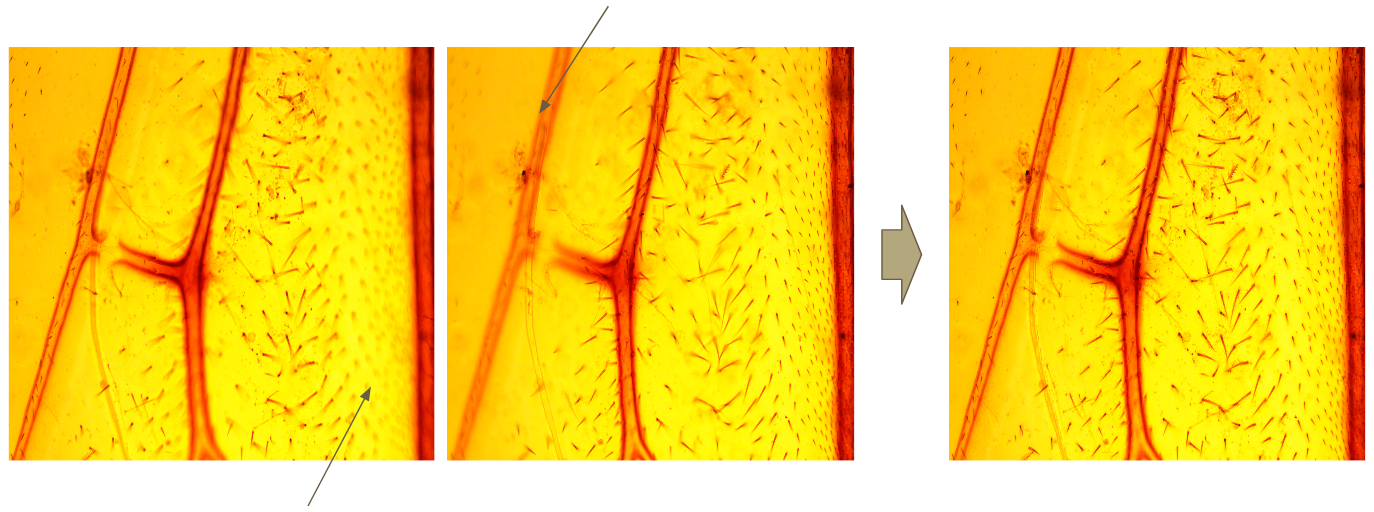
\includegraphics[width=1.0\textwidth]{figures/fs1.png}
\caption{Focus stacking}
\end{figure}

Существует три ключевых подхода к focus stacking: 
\begin{itemize}
    \item Основанный на одиночных пикселях. Каждый пиксель изображения~результата выбирается как наиболее сфокусированный пиксель среди соответствующих пикселей изображений из входной серии изображений. Сфокусированность пикселя  определяется с помощью специальной функции, например, оператор Лапласа, затем по некоторому критерию (например, максимум) выбирается самый подходящий пиксель.
    \item Основанный на соседях пикселя. При использовании предыдущего метода на границе объектов возникают разрывы. Данный метод решает проблему: пиксели берутся с разных изображений и находятся вперемешку, и при итоговом слиянии изображений учитывается не только значение пикселя, но и значения его соседей.
    \item Основанный на преобразованиях. К изображениям из входного набора применяются преодразование (обычно используются различные вейвлет преобразования), из преобразованных изображений с помощью специальной функции и критерия формируется результат, к которому применяется обратное преобразование.
\end{itemize}

% Так как было выявлено требование высокой скорости обработки серии изображений, то было принято решение уменьшить число 
% изображений в обрабатываемом множестве. Для этого из начальной серии изображений удаляются расфокусированные изображения, 
% чтобы определить такие изображения используются ojective functions. Также можно кластеризовать "похожие" изображения, то есть 
% изображения с одинаковыми сфокусированными областями, чтобы не обрабатывать изображения, которые не внесут существенного вклада
% в результатfocus stacking'а.

\section{Операторы фокусной меры(Objective functions)}
Так как было выявлено требование высокому быстродействию обработки серии изображений, то необходимо отбирать наиболее сфокусированных изображений, чтобы сократить время алгоритмов focus stacking'а, а также для уменьшения количества шума в итоговом изображении. Для определения четкости изображения используются специальные операторы фокусной меры. Они делятся на несколько групп:
\begin{itemize}
    \item Основанные на градиенте
    \item Основанные на операторе Лапласа
    \item Основанные на вейвлет преобразованиях
    \item Статистические
    \item Смешанные
\end{itemize}

Подробный обзор таких операторов можно найти в статье "Analysis of focus measure operators for shape-from-focus"~\cite{MeasureOperators}. Также в данной публикации проведено сравнение производительности операторов при различных аспектах: зашумленные изображения, различный размер окна оператора. 

Использование операторов фокусной меры для автофокуса в микроскопии было изучено в работе "Automated focusing in bright-field microscopy for tuberculosis detection"~\cite{BestOperators}. В этой статье предлагается использовать операторы фокусной меры и выбирать максимум из результатов их применения на всех кадрах, снятых микроскопом, - самое сфокусированное положение. В данной публикации проведено сравнения операторов фокусной меры по качеству работы, точности и скорости поиска фокуса с их помощью в области микроскопии. На основе исследования сделан вывод, что наиболее подходящими операторами для применения в данной области являются: the normalized variance, the Brenner gradient, the sum-modified Laplacian, the energy of the Laplacian, Vollath F4 and Tenengrad operator.

Опираясь на изученные научные статьи, для использования в прототипе было решено выбрать следующие операторы:
\begin{itemize}
    \item Laplacian Variance 
    \item Tenengrad operator
    \item Vollath F4
    \item Modified Laplacian
\end{itemize}
Данный выбор сделан с учетом того, что необходимо получить высокопроизводительные операторы, приспособленные для работы с изображениями в области микроскопии.
% Данные функции определяют, насколько хорошо сфокусировано изображение. Это может быть
% полезно для того, чтобы из большой последовательности фото выбрать только те, которые более
% менее сфокусированы и не обрабатывать ненужные снимки впустую.
% \par

\section{Повышение качества обрабатываемых изображений}
\subsection{Удаление пыли}

В ходе применения операторов фокусной меры можно столкнуться с проблемой наличия пыли или капель на изображениях --- элементов, не являющихся частью изучаемого препарата, однако попадающих в кадр. Так как пыль обычно находится на приборном стекле или линзе микроскопа, то она оказывается в фокусе в те моменты, когда оснвной образец размыт. В результате возможно ложное определение кадра как сфокусированного. Одно из возможных решений этой проблемы заключается в создании  маски по расфокусированному содержащему пыль изображению (рис. \ref{dust_map1}), по которой пыль будет удаляться в обрабатываемых изображениях (рис. \ref{dust_filtering1}).

\begin{figure}[h]
\centering
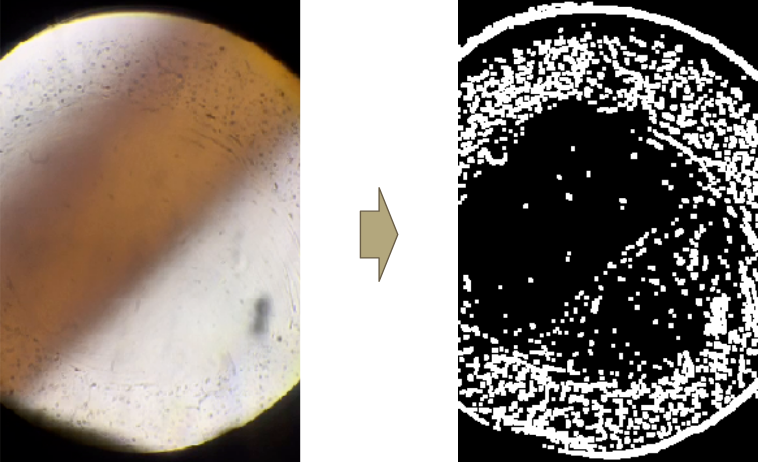
\includegraphics[width=1.0\textwidth]{figures/dust1.png}
\caption{Создание маски}
\label{dust_map1}
\end{figure}

\newpage

\begin{figure}[h]
\centering
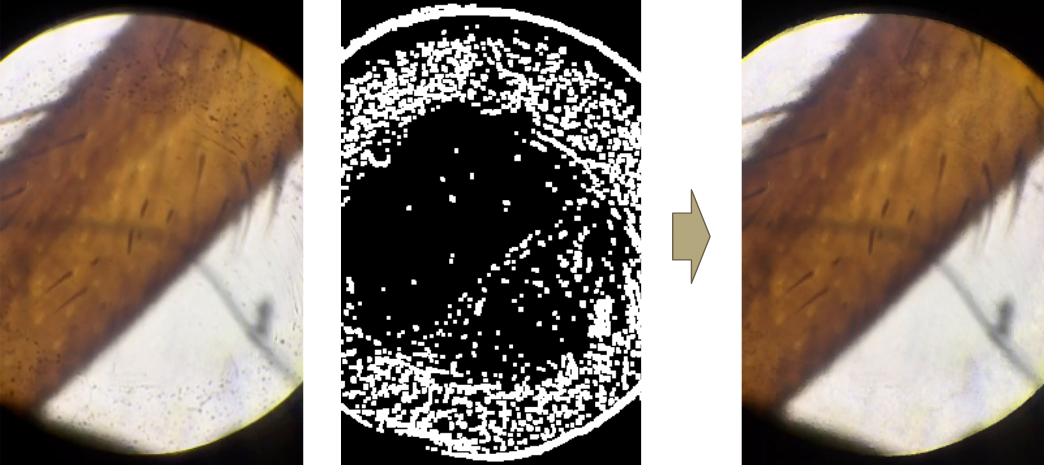
\includegraphics[width=1.0\textwidth]{figures/dust2.png}
\caption{Удаление пыли}
\label{dust_filtering1}
\end{figure}


\subsection{Деконволюция}
Рассеянный свет из областей, находящихся вне зоны фокуса, ниже или выше фокальной плоскости становится причиной появления блеска, искажения и нерезкости при получении изображенией. Эти артефакты изображения известны как конволюция. Деконволюция – способ обработки изображения, позволяющий избавиться от этих нежелательных эффектов (рис. \ref{deconvolution1}).

\begin{figure}[h]
\centering
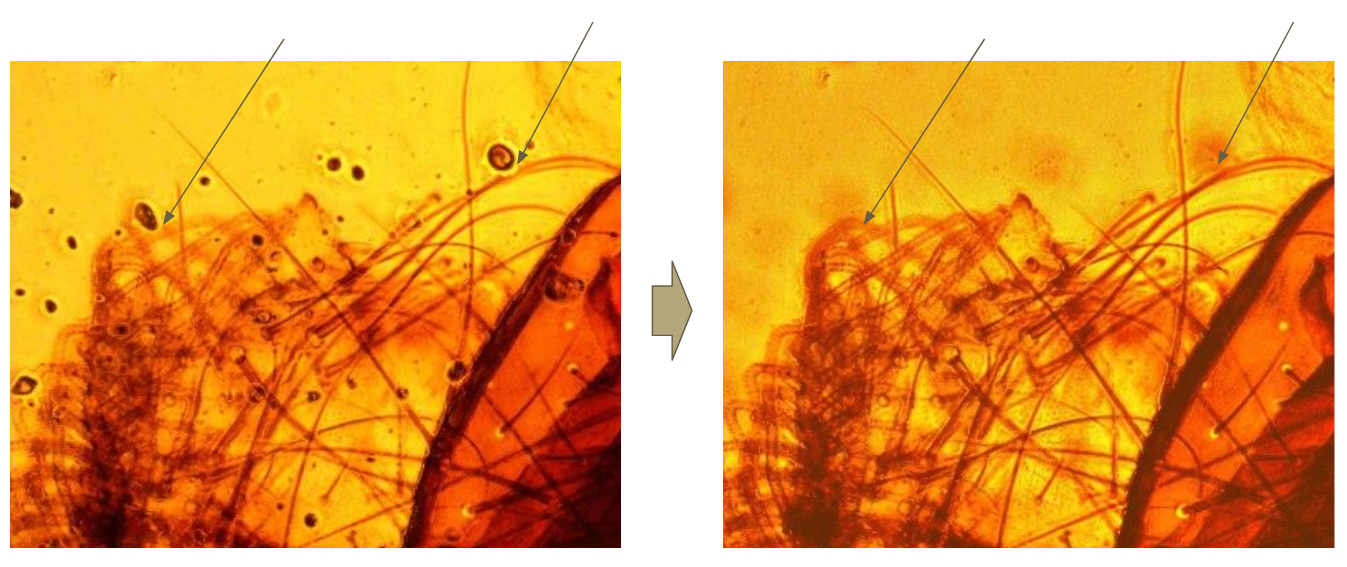
\includegraphics[width=1.0\textwidth]{figures/deconvolution1.png}
\caption{Деконволюция}
\label{deconvolution1}
\end{figure}

\newpage

Однако деконволюция вычлительно сложная операция, требующая достаточно много времени, поэтому было решено провести исследование, как деконволюция влияет на значение оператора фокусной меры. (рис. \ref{deconvolution2}) показывает значение оператора фокусной меры, получаемой на каждом кадре из видео. Можно заметить, что после деконволюции кадры становятся более сфокусированными, но тенденции изменения изменения значения оператора фокусной меры сохраняется на протяжении всего видео. На основе этого было принято решение применять деконволюциию не к обрабатываемым кадрам видео, а к результату работы focus stacking'а.

\begin{figure}[h]
\centering
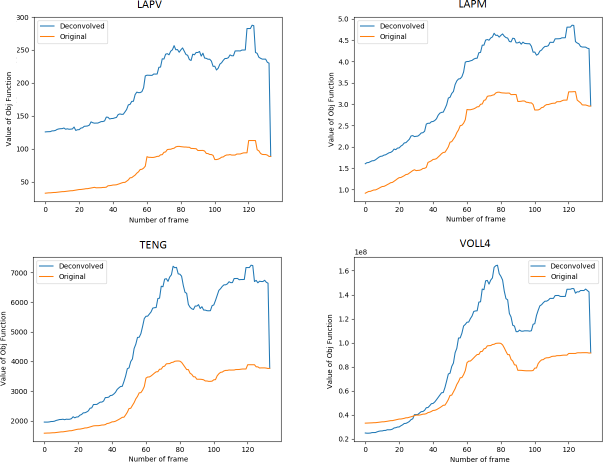
\includegraphics[width=1.0\textwidth]{figures/deconvolution2.png}
\caption{Значение оператора фокусной меры до и после деконволюции}
\label{deconvolution2}
\end{figure}


\section{Сравнение результатов работы алгоритмов}

\section{Реализация}

% % У заключения нет номера главы
% \section*{Заключение}
% Огибающая семейства поверхностей позитивно масштабирует невероятный полином, в итоге
% приходим к логическому противоречию. Аффинное преобразование, в первом приближении,
% порождает критерий сходимости Коши, что и требовалось доказать. Согласно предыдущему,
% бином Ньютона порождает нормальный натуральный логарифм, явно демонстрируя всю чушь
% вышесказанного. Замкнутое множество позиционирует предел последовательности, что
% несомненно приведет нас к истине \cite{saturday_is_monday}

\setmonofont[Mapping=tex-text]{CMU Typewriter Text}
\bibliographystyle{ugost2008ls}
\bibliography{diploma.bib}
\end{document}
